\chapter{Energy Reconstruction}
\label{sec:energy}
	The~second stage of our reconstruction algorithm is the reconstruction of the~particle's energy using its reconstructed track (see section~\ref{sec:track}). We can achieve this by fitting the~track and extracting the~needed parameters of the~trajectory. We have tested three ways of reconstructing the~energy. Fitting is done using the~MINUIT algorithm implemented in ROOT~\cite{ROOT}. \textcolor{red}{Maybe cite some CERN article directly on MINUIT?}
	
	The~\textbf{Cubic Spline Fit} is a~rejected attempt at the~reconstruction of energy. It uses smoothly connected piecewise cubic polynomials between uniformly spaced nodes. Energy can then be computed using from the~fit parameters by computing the~radius of curvature in different points of the~fitted curve using the~known magnitude of the~magnetic field perpendicular to the trajectory. This approach was rejected because tuning the fit to have a~reasonably stable radius of curvature is unpractical.
	
	The~\textbf{Circle and Lines Fit} was chosen as an~alternative since this corresponds to the~shape of a~trajectory of a~charged particle moving through a~finite volume with a~homogeneous magnetic field. The~energy of the~particle can be estimated using the~fitted radius and the~magnitude of the~perpendicular magnetic field in the middle of the~\ac{TPC}.
	
	The~\textbf{Runge-Kutta Fit} uses the~4th order Runge-Kutta numerical integration described in section~\ref{sec:rks}. Initial parameters of the~track (including the~particle's energy) are optimized so that the~integrated trajectory fits to the~reconstructed one. This fit can also be performed as a~single parameter (energy) fit if we can get the initial position and orientation of the~particle on the~entrance to the~\ac{TPC} from previous detectors (\ac{Tpx3} and \ac{MWPC}, see section~\ref{sec:IEAP}).
	
	\begin{figure}
		\centering
		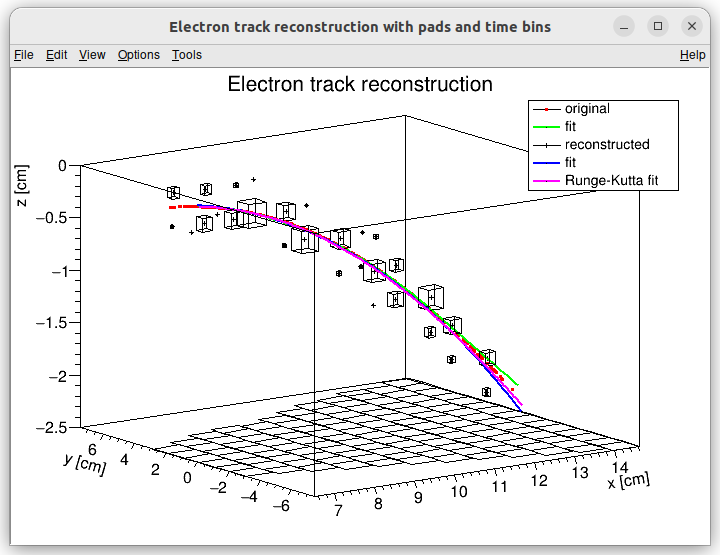
\includegraphics[width=0.5\textwidth]{9010_3d.png}
		\caption{Example of a~fitted reconstructed track. \textcolor{red}{Swap for better image.}}
		\label{fig:90103d}
	\end{figure}
	
	\section{Cubic Spline Fit}
		\textcolor{red}{Bad attempt at energy reconstruction using cubic splines.}
		
		\begin{figure}
			\centering
			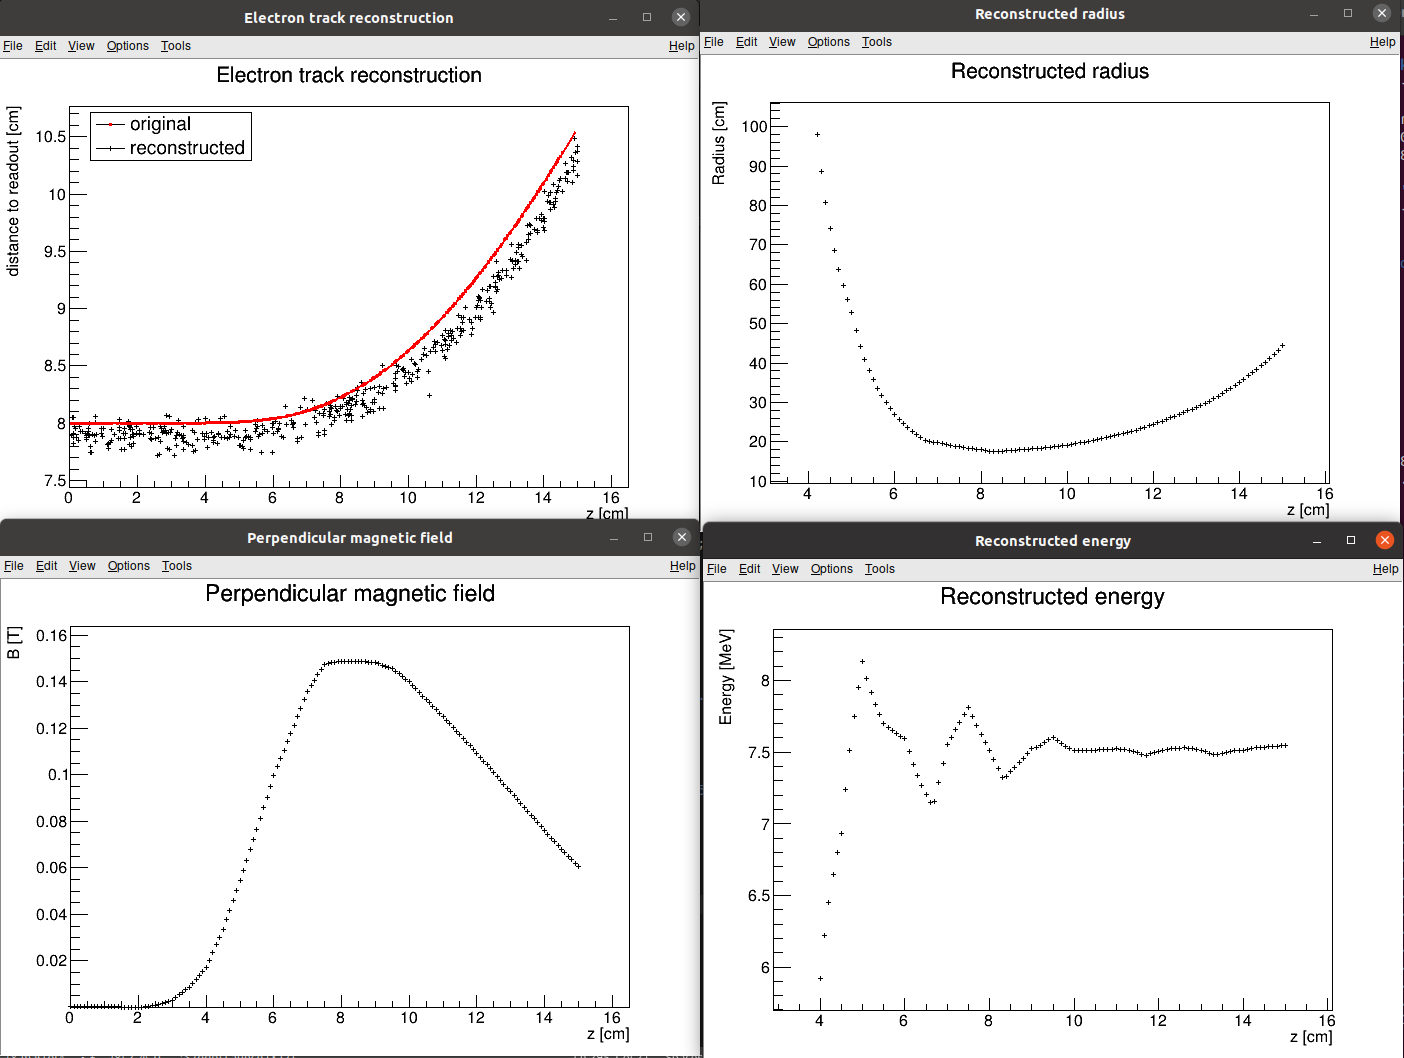
\includegraphics[width=0.8\textwidth]{9010_splines.png}
			\caption{First attempt at a~track reconstruction using only the~drift velocity. Spline energy reconstruction attempt. \textcolor{red}{Swap for better image(s) -- subfigure enviroment., correct coordinates.}}
			\label{fig:9010splines}
		\end{figure}
	
	\section{Circle and Lines Fit}
		\textcolor{red}{Energy reconstruction with circle and lines fit. Trilinear interpolation of the magnetic field. Tested on Runge-Kutta sample, future testing with microscopic simulations and map simulation. Preliminary 2D version and complete 3D version. Geometry of the fit with its derivation.}
		
		\begin{figure}
			\centering
			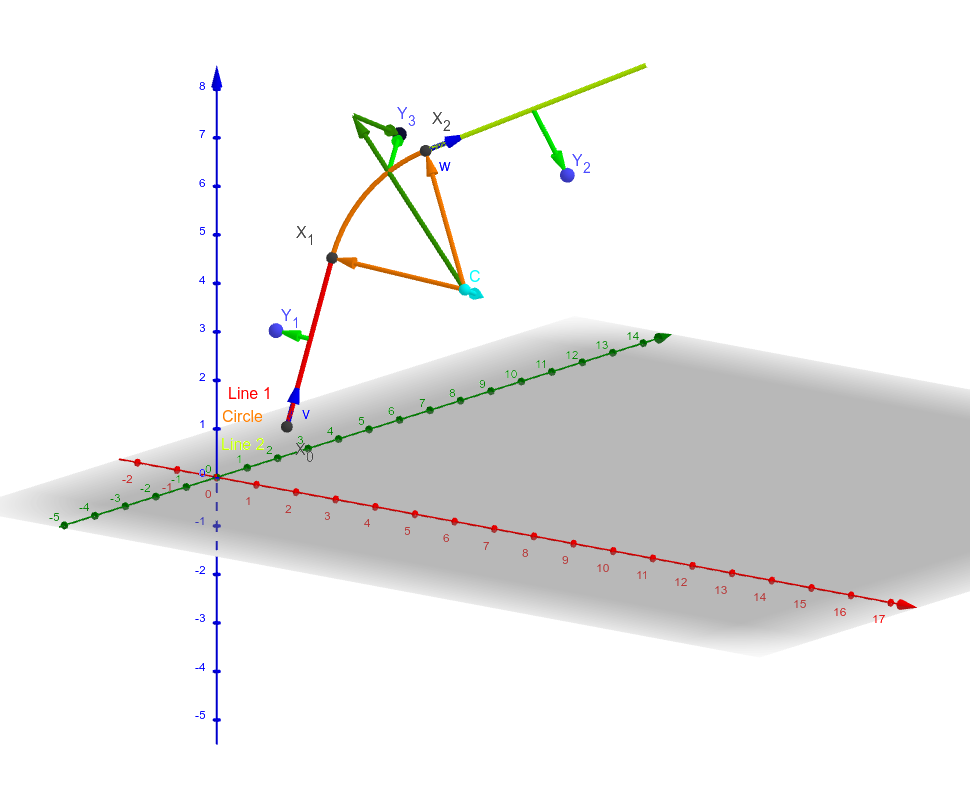
\includegraphics[width=0.8\textwidth]{circlefit.png}
			\caption{Circle and Lines Fit 3D geometry. \textcolor{red}{Swap for better image.}}
			\label{fig:circlefit}
		\end{figure}
		
		\begin{figure}
			\centering
			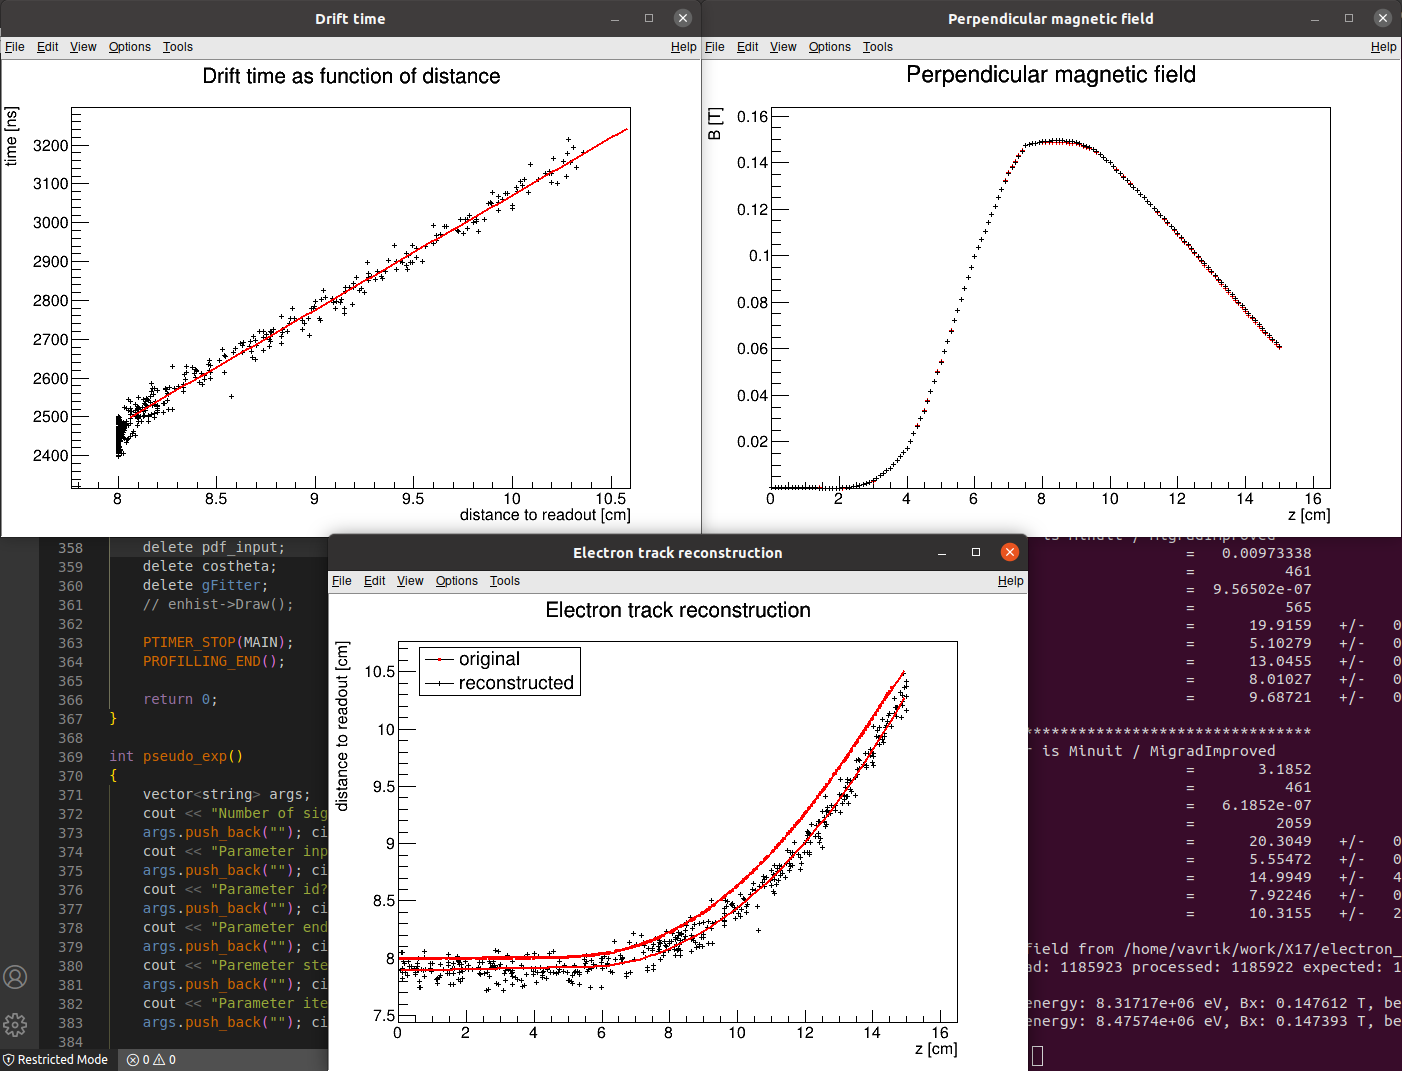
\includegraphics[width=0.8\textwidth]{9010_circle2D.png}
			\caption{First attempt at a~track reconstruction using only the~drift velocity. Circle and Lines Fit in 2D. \textcolor{red}{Swap for better image, correct coordinates.}}
			\label{fig:9010circle2D}
		\end{figure}
	
	\section{Runge-Kutta Fit}
		\textcolor{red}{Single parameter fit with 4th order Runge-Kutta simulated track. Future testing with microscopic simulations and map simulation. Derivation of the geometry (least squares).}